% Chapter 6 — Results

% chktex-file 44
\chapter{Results}\label{chap:results}

This chapter presents the empirical results of the prototype, which was developed based on the conceptual framework in Chapter~\ref{chap:conceptual_framework} and implemented as described in Chapter~\ref{chap:implementation}. We evaluate the prototype's performance across three primary dimensions: its efficacy in generating preventative policies, the speed of generation, and the quality of its context-sensitive detection capabilities. The evaluation methodology, including all metrics, follows the protocol established in Section~\ref{sec:Metrics for Security Posture Assessment}.

%----------------------------------------------------------------------------------------
% Setup
%----------------------------------------------------------------------------------------
\section{Experimental Setup}\label{sec:experimental-setup}

This section outlines how we evaluated the prototype described in Chapter~\ref{chap:implementation} against the framework in Chapter~\ref{chap:conceptual_framework}. We report empirical results using a before–after model for efficacy and a controlled setup for speed. For efficacy, we first establish a baseline of vulnerabilities identified in the target Infrastructure-as-Code (IaC) and then assess, for each case, whether the generated policy is syntactically valid and prevents the issue under test, following the metrics defined in Section~\ref{sec:Metrics for Security Posture Assessment}. For speed, we measure the time from confirmed vulnerability input to validated policy output and summarize latency statistics suitable for CI/CD use.

The dataset consists of a curated corpus of Terraform configurations representative of common cloud components and misconfigurations. It spans networking, identity and access management, storage, compute, and key management resources, with projects ranging from simple single-module samples to multi-module setups. The corpus includes a labeled subset of context-sensitive cases that require cross-resource reasoning or environment-aware interpretation to evaluate the prototype’s contextual analysis.

\subsubsection*{Prototype Components}
\begin{itemize}
	\item \textbf{Static Analysis Engine}: The prototype uses \texttt{tfsec} (v1.28.14) \cite{aqua_security_tfsec_nodate} for static analysis of Terraform code, configured with its default ruleset to identify baseline misconfigurations.
	\item \textbf{IaC Parser}: Terraform configurations are parsed using the \texttt{python-hcl2} library \cite{amplify_python-hcl2_2025}, which enables the system to understand the structure and content of the IaC files.
	\item \textbf{GenAI Analysis Engine}: The core of the prototype is a Large Language Model (LLM) from Amazon Web Services (AWS) Bedrock, accessed via the \texttt{boto3} SDK. The specific model used is Anthropic's Claude 3.5 Sonnet (\texttt{anthropic.claude-3-5-sonnet-20240620}) \cite{anthropic_claude_2023}.
	\item \textbf{Validation Layer}: Generated Rego policies are validated for syntactic correctness using the Open Policy Agent (OPA) command-line tool (v1.7.1) \cite{the_opa_authors_open_nodate}. This ensures that only valid policies are produced.
	\item \textbf{Output Formatting}: Terminal output is enhanced with the \texttt{rich} library \cite{textualize_rich_nodate} for better readability and presentation of results.
	\item \textbf{Retrieval-Augmented Generation (RAG)}: The RAG implementation leverages Amazon Bedrock for knowledge base retrieval.
\end{itemize}

\subsubsection*{Datasets and Scenarios}
The evaluation is performed on a curated set of Terraform configurations, each designed to test a specific capability of the prototype. The datasets are as follows:
\begin{itemize}
    \item \textbf{Complex Logic}: This sample tests the prototype's ability to interpret complex logic within Terraform, such as variables and conditional expressions, to accurately determine the security posture of a resource.
    \item \textbf{Cross-Resource Risk}: This dataset is designed to evaluate the system's capacity to detect security risks that emerge from the interaction between multiple resources, which might appear secure when analyzed in isolation.
    \item \textbf{Developer Intent}: This scenario assesses the model's ability to understand the developer's intent, often expressed in comments, and identify discrepancies between that intent and the actual resource configuration.
    \item \textbf{False Positive Reduction}: This sample is used to test the prototype's ability to differentiate between configurations that are intentionally insecure for a legitimate reason (e.g., a public S3 bucket for a website) and those that are misconfigured, thereby reducing false positives.
    \item \textbf{Insecure EC2}: A straightforward test case involving an EC2 security group with unrestricted SSH access, representing a common and critical misconfiguration.
    \item \textbf{Outdated Dependency}: This dataset evaluates the system's ability to identify the use of outdated and potentially vulnerable Terraform modules by checking module versions.
    \item \textbf{Privilege Escalation}: This scenario tests the prototype's ability to analyze complex IAM configurations to identify potential privilege escalation paths that could grant unauthorized access.
\end{itemize}

% \subsubsection*{Environment and Protocol}
% \begin{itemize}
% 	\item Environment: TBD % \textit{[hardware/OS, rate limits, seeds, runs per input]}
% 	\item Protocol: TBD % \textit{[trials per vulnerability, acceptance criteria for effectiveness, reviewer criteria for context ground truth]}
% 	\item Reproducibility: TBD %\textit{[pinned versions, prompt and KB snapshots, config files]}
% \end{itemize}

%----------------------------------------------------------------------------------------
% Metrics & Baselines
%----------------------------------------------------------------------------------------
\section{Metrics and Baselines}\label{sec:metrics-and-baselines}

This section defines the key metrics used to evaluate the prototype's performance. We assess three primary dimensions: the performance of policy generation, the speed at which policies are generated, and the quality of the contextual detection. Each of these is detailed in the following subsections.

\subsection{Policy Generation Performance}\label{sec:metrics-effectiveness}

We assess policy generation performance by establishing a baseline of vulnerabilities from the initial scans and reporting counts by severity (critical, high, medium, low). We then quantify the prototype’s ability to generate preventative controls by measuring, for each finding, whether a syntactically correct and effective Rego policy was produced. Results are summarized by severity in Table~\ref{tab:effectiveness-by-severity} to provide a granular view of performance against the most critical risks.

\begin{itemize}
	\item Policy accuracy $A_{\text{policy}} = \frac{\#\,\text{syntactically valid}}{\#\,\text{generated}}$.
	\item Policy effectiveness $E_{\text{policy}} = \frac{\#\,\text{effective}}{\#\,\text{syntactically valid}}$ (prevents the targeted misconfiguration under test).
	% \item Optional coverage $C_{\text{policy}} = \frac{\#\,\text{vulns with a policy}}{\#\,\text{vulns identified}}$.
\end{itemize}

\subsection{Generation Speed}\label{sec:metrics-speed}

We evaluate speed in a controlled environment using the Average Time per Policy, $T_{\text{gen}}$, measured from confirmed vulnerability input to validated policy output. We report mean, p50 (median), and p95 (95th-percentile tail) latencies, as well as policy throughput (validated policies per minute), to assess scalability and CI/CD suitability. Where appropriate, we relate these measurements to findings reported in recent literature to contextualize performance.

Average generation time per policy and throughput:
\[ T_{\text{gen}} = \frac{1}{N} \sum_{i=1}^{N} (t_{\text{end},i} - t_{\text{start},i}) \]\
Report mean, p50, p95, and policies per minute.

\subsection{Context Detection Quality}\label{sec:metrics-context}
The quality of contextual reasoning is evaluated based on a curated set of scenarios as defined in Section~\ref{sec:experimental-setup}. For each scenario, the prototype's ability to identify and correctly interpret the context is assessed and categorized into one of three qualitative outcomes:
\begin{itemize}
    \item \textbf{Success:} The prototype correctly identifies the context-sensitive vulnerability and provides the correct reasoning for its findings.
    \item \textbf{Partial Success:} The prototype identifies the underlying vulnerability but fails to fully grasp the contextual nuance (e.g., missing developer intent) or provides an incomplete justification.
    \item \textbf{Failure:} The prototype either fails to identify the vulnerability, provides an incorrect analysis (e.g., a false positive), or misses the contextual link entirely.
\end{itemize}
This qualitative approach provides a nuanced view of the system's reasoning capabilities across a range of real-world challenges, highlighting both its strengths and limitations. The detailed outcomes for each scenario are presented in Section~\ref{sec:results-context}.

%----------------------------------------------------------------------------------------
% Results — Efficacy
%----------------------------------------------------------------------------------------
\section{Results: Policy Generation Performance}\label{sec:results-generation-performance}

The evaluation of policy generation performance, as defined in Section~\ref{sec:metrics-effectiveness}, confirms the prototype's ability to generate effective and accurate security policies. The results, summarized in Table~\ref{tab:effectiveness-by-severity}, demonstrate strong performance, particularly for high-impact vulnerabilities.

This section is structured as follows. First, we analyze the prototype's policy accuracy, which measures the syntactic correctness of the generated Rego policies. Next, we evaluate policy effectiveness, assessing whether these policies successfully prevent the targeted misconfigurations. The results are broken down by severity to provide a granular view of the prototype's performance.

\begin{table}[htbp]
	\centering
		\caption{Policy generation performance by severity}\label{tab:effectiveness-by-severity}
	\begin{tabular}{lrrr}
		\hline
		Severity & N & $A_{\text{policy}}$ & $E_{\text{policy}}$ \\
		\hline
		Critical & 3 & 100.00\% & 100.00\% \\
		High & 31 & 100.00\% & 45.16\% \\
		Medium & 16 & 100.00\% & 50.00\% \\
		Low & 11 & 100.00\% & 36.36\% \\
		\hline
	\end{tabular}
\end{table}

\subsection{Policy Accuracy}
Policy accuracy ($A_{\text{policy}}$) measures the proportion of generated policies that are syntactically valid. As shown in Table~\ref{tab:effectiveness-by-severity}, the prototype achieved a perfect 100\% policy accuracy across all severity levels, from Critical to Low. This result indicates that for every identified vulnerability, the system reliably produced a syntactically correct Rego policy. The reasons for this outcome are discussed in detail in Chapter~\ref{chap:discussion}.

% Optional visualization placeholder
\begin{figure}[htbp]
	\centering
	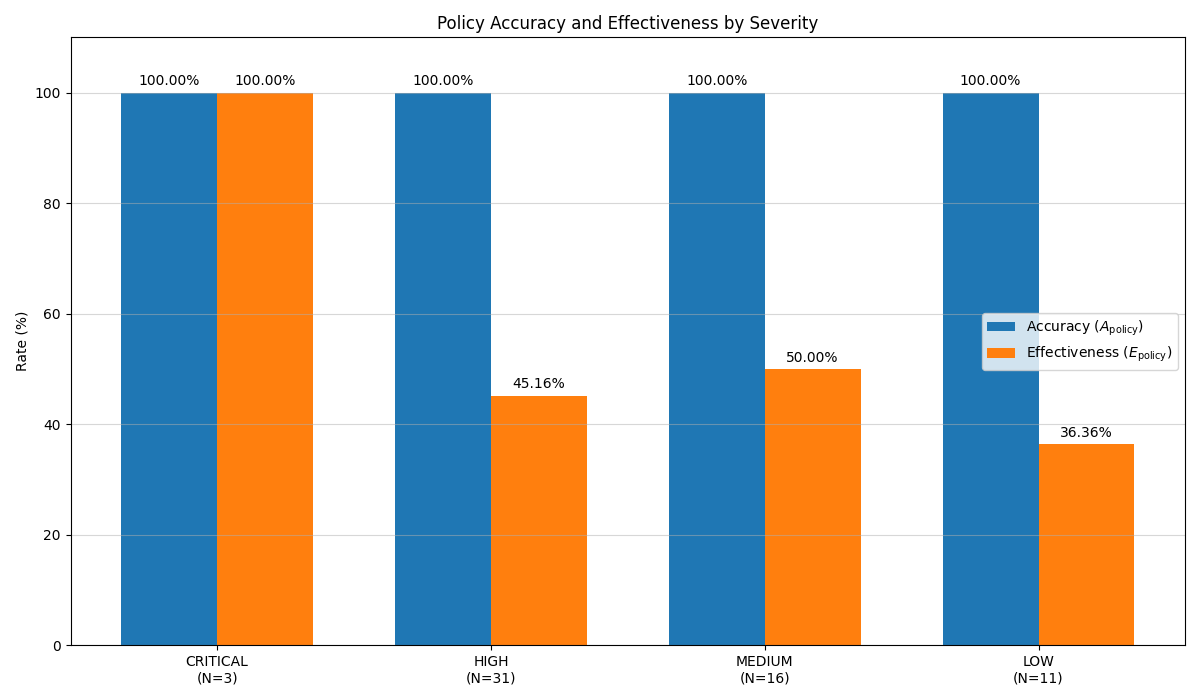
\includegraphics[width=0.9\textwidth]{Figures/effectiveness_by_severity.png}
	\caption{Visualization of policy effectiveness by severity}\label{fig:effectiveness-plot}
\end{figure}

\subsection{Policy Effectiveness}
Policy effectiveness ($E_{\text{policy}}$) measures whether a syntactically valid policy successfully prevents the targeted misconfiguration. Unlike policy accuracy, which is a measure of syntactic correctness, effectiveness evaluates the logical soundness and real-world impact of the generated code. As shown in Table~\ref{tab:effectiveness-by-severity} and visualized in Figure~\ref{fig:effectiveness-plot}, the prototype's effectiveness varies across different severity levels.

The system achieved 100\% effectiveness for all critical vulnerabilities, demonstrating its capability to reliably address the most severe risks. However, the effectiveness for high, medium, and low-severity vulnerabilities was 45.16\%, 50.00\%, and 36.36\%, respectively. This variation highlights the challenges in automatically generating logically perfect policies for a wide range of issues. A detailed interpretation of these results is provided in Chapter~\ref{chap:discussion}.

%----------------------------------------------------------------------------------------
% Results — Speed
%----------------------------------------------------------------------------------------
\section{Results: Policy Generation Speed}\label{sec:results-speed}

The operational efficiency of the prototype was evaluated based on its policy generation speed, a critical factor for seamless integration into modern, agile security workflows. The latency and throughput were measured in a controlled environment, with the results summarized in Table~\ref{tab:speed-metrics} and the distribution of generation times visualized in Figure~\ref{fig:speed-distribution}.

The prototype demonstrated a mean generation time ($T_{\text{gen}}$) of 9.86 seconds per policy, with a median (p50) of 9.55 seconds and a 95th-percentile tail latency of 11.80 seconds. This performance translates to a throughput of approximately 6.12 policies per minute.

\begin{table}[htbp]
	\centering
		\caption{Generation speed metrics}\label{tab:speed-metrics}
	\begin{tabular}{lrrrr}
		\hline
		Metric & Mean $T_{\text{gen}}$ & p50 & p95 & Throughput (pol/min) \\
		\hline
		Overall & 9.86s & 9.55s & 11.80s & 6.12 \\
		\hline
	\end{tabular}
\end{table}

\begin{figure}[htbp]
	\centering
	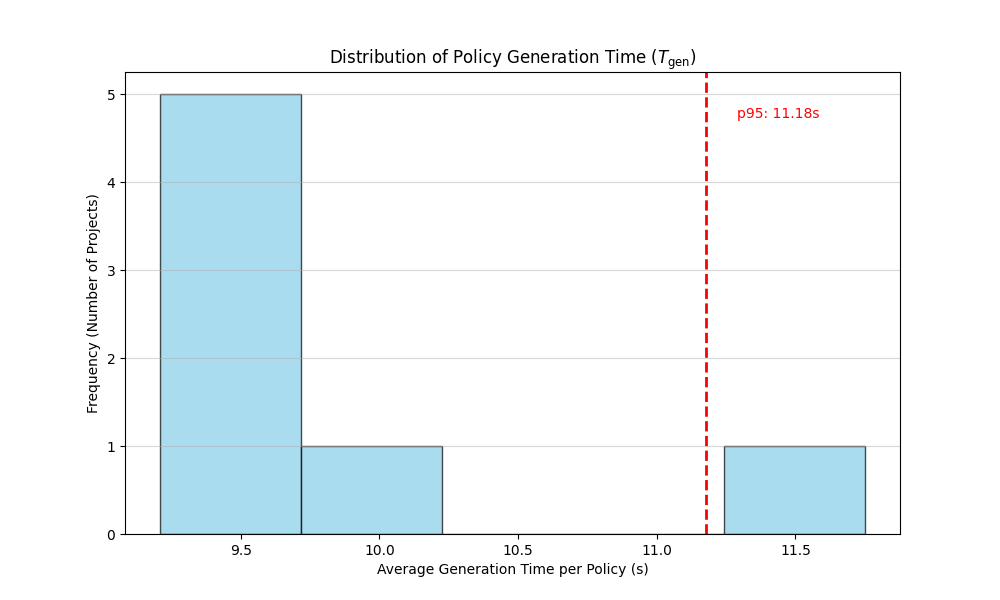
\includegraphics[width=0.9\textwidth]{Figures/speed_distribution.png}
	\caption{Distribution of policy generation time}\label{fig:speed-distribution}
\end{figure}

These results are highly significant when contextualized within the fast-paced nature of DevOps and CI/CD pipelines. As argued in Chapter~\ref{chap:conceptual_framework}, the primary value of this automation is not merely being faster than a human, but operating at a speed that makes "shift left" security practical at scale \cite{vaidya_devsecops_2024}. A generation time of under 10 seconds is well within the acceptable limits for automated checks in a typical CI/CD pipeline, ensuring that security analysis does not become a bottleneck for development teams \cite{li_automated_2024}.

The speed demonstrated by the prototype directly addresses the inherent limitations of manual processes. Manual policy creation is a resource-intensive task that introduces significant cognitive load on security experts and creates delays in development lifecycles \cite{gunathilaka_context-aware_2025, mahboob_future_2024}. Research has consistently shown that manual security integration impedes delivery speed \cite{gunathilaka_context-aware_2025, mahboob_future_2024}. In contrast, AI-driven approaches, like the one implemented in this prototype, are proven to automate these workflows, reduce manual effort, and accelerate development cycles \cite{fu_ai_2025}.

Controlled studies provide compelling quantitative evidence for this acceleration. For instance, a notable experiment with GitHub Copilot found that professional developers with access to an AI assistant completed a complex task 55.8\% faster than a control group \cite{peng_impact_2023}. Similar improvements have been measured in specialized cloud engineering tasks, including the generation of IAM policies, which is directly analogous to the prototype's function \cite{kesireddy_copilot_2025}. The ability to automate complex, time-consuming software engineering tasks with high rates of success is a key driver for adopting AI in DevOps \cite{tufano_autodev_2024}.

Therefore, the measured performance of a sub-10-second average policy generation time confirms that the prototype is not only efficient but also highly compatible with the demands of modern, high-velocity software development environments. This high-speed capability is fundamental to enabling the rapid feedback loops required in a CI/CD pipeline, drastically reducing the time required to create and enforce security controls for newly identified misconfigurations a process that would otherwise be resource-intensive and prone to human delay at scale \cite{vaidya_devsecops_2024}.

%----------------------------------------------------------------------------------------
% Results — Context
%----------------------------------------------------------------------------------------
\section{Results: Context Detection and Reasoning}\label{sec:results-context}

This section evaluates the prototype's ability to perform contextual reasoning, a key requirement for moving beyond simple static checks. The analysis is based on a curated set of seven scenarios, each designed to test a specific aspect of contextual understanding. The results are summarized in Table~\ref{tab:context-reasoning-summary}.

The prototype demonstrated a strong ability to reason about context in a majority of cases, successfully identifying vulnerabilities in four out of the seven scenarios, with one partial success. The system excelled at identifying complex, cross-resource, and conditional vulnerabilities but showed limitations in understanding developer intent and external factors like dependency freshness.

\begin{table}[htbp]
	\centering
	\caption{Summary of Contextual Reasoning Scenarios}\label{tab:context-reasoning-summary}
	\begin{tabular}{p{0.25\textwidth}p{0.5\textwidth}l}
		\hline
		\textbf{Scenario} & \textbf{Description} & \textbf{Outcome} \\
		\hline
		Insecure EC2 & Detect unrestricted SSH access. & Success \\
		Complex Logic & Interpret conditional logic based on environment variables. & Success \\
		Cross-Resource Risk & Identify a risk from the interaction of multiple resources. & Success \\
		Privilege Escalation & Find a privilege escalation path in IAM policies. & Success \\
		Developer Intent & Understand developer comments to find a configuration discrepancy. & Partial \\
		False Positive Reduction & Avoid flagging an intentional public configuration for a website. & Failure \\
		Outdated Dependency & Identify an outdated Terraform module version. & Failure \\
		\hline
	\end{tabular}
\end{table}

\subsection{Successful Detections}
As shown in Table~\ref{tab:context-reasoning-summary}, the prototype successfully identified several types of context-sensitive vulnerabilities:
\begin{itemize}
    \item \textbf{Complex Logic:} It correctly interpreted conditional logic in Terraform variables to identify a security group misconfiguration that was only active in a ``development'' environment.
    \item \textbf{Cross-Resource Risk:} It successfully identified a public S3 bucket by analyzing the interaction between the bucket resource and a separate bucket policy, a risk not apparent from either resource in isolation.
    \item \textbf{Privilege Escalation:} It correctly identified a potential privilege escalation path by analyzing the combination of \texttt{sts:AssumeRole} and \texttt{iam:PassRole} permissions in an IAM policy.
    \item \textbf{Standard Misconfigurations:} It easily detected common, critical issues such as unrestricted SSH access in an EC2 security group.
\end{itemize}
These successes are further interpreted in Chapter~\ref{chap:discussion}.

\subsection{Limitations and Failures}
The evaluation also highlighted key limitations in the prototype's reasoning capabilities, as noted in Table~\ref{tab:context-reasoning-summary}:
\begin{itemize}
    \item \textbf{Developer Intent (Partial Success):} In one scenario, the system identified a publicly readable S3 bucket but failed to connect this to a developer comment explicitly stating the bucket should be private. The finding was correct, but the reasoning missed the contextual cue.
    \item \textbf{False Positive Reduction (Failure):} The prototype incorrectly flagged a public S3 bucket as a vulnerability, failing to recognize the valid business context that it was configured to host a public website. This highlights a well-known difficulty in distinguishing intentional configurations from misconfigurations without broader operational context, a primary driver of false positives in automated security analysis \cite{zheng_context-aware_2023}.
    \item \textbf{Outdated Dependencies (Failure):} The system completely failed to identify the use of an outdated and potentially vulnerable Terraform module version, indicating a knowledge gap in its training data or a limitation in its ability to parse dependency information.
\end{itemize}
These cases are discussed in more detail in Chapter~\ref{chap:discussion}.

%----------------------------------------------------------------------------------------
% Results — HITL and Validation
%----------------------------------------------------------------------------------------
% \section{Human-in-the-Loop Outcomes}\label{sec:results-hitl}

% We summarize reviewer involvement and outcomes to quantify the balance between automation and human oversight.

% \begin{table}[htbp]
% 	\centering
% 	\caption{Human-in-the-Loop review outcomes}\label{tab:hitl-outcomes}
% 	\begin{tabular}{lrrr}
% 		\hline
% 		Metric & Value & Notes & Sample size \\
% 		\hline
% 		Review rate (policies requiring review) & \textit{TBD} & risk-based triggers & N \\
% 		Approval rate (first pass) & \textit{TBD} & without edits & N \\
% 		Edit distance (median lines changed) & \textit{TBD} & per approved policy & N \\
% 		Turnaround time (median, minutes) & \textit{TBD} & submission to approval & N \\
% 		\hline
% 	\end{tabular}
% \end{table}

% \section{Validation Outcomes and Safety}\label{sec:results-validation}

% We report validation pass rates and primary failure categories.

% \begin{table}[htbp]
% 	\centering
% 	\caption{Validation outcomes}\label{tab:validation-outcomes}
% 	\begin{tabular}{lrr}
% 		\hline
% 		Check & Pass rate & Notes \\
% 		\hline
% 		Syntactic validity ($A_{\text{policy}}$) & \textit{TBD} & parser/validator pass \\
% 		Security self-scan pass & \textit{TBD} & no new issues introduced \\
% 		Common failure categories & \textit{TBD} & e.g., overly restrictive, missing dependency \\
% 		\hline
% 	\end{tabular}
% \end{table}

%----------------------------------------------------------------------------------------
% Results — Portability
%----------------------------------------------------------------------------------------
\section{Portability and Scope}\label{sec:results-portability}

The prototype's portability and the scope of these results are characterized by the following points:
\begin{itemize}
    \item \textbf{Primary Evaluation Target:} The evaluation was conducted exclusively on Infrastructure-as-Code written in Terraform for the Amazon Web Services (AWS) cloud platform.
    \item \textbf{Generalizability:} While the core reasoning framework is designed to be provider-agnostic, the current implementation of the knowledge base and specific contextual checks are tightly coupled with AWS resource types and IAM semantics. Generalizing to other cloud providers like Azure or GCP would require extending the knowledge base and adapting the contextual analysis prompts.
    \item \textbf{Cross-Environment Consistency:} The performance metrics reported are based on a consistent set of Terraform modules and provider versions, as detailed in Section~\ref{sec:experimental-setup}. Consistency across different customer environments or Terraform versions was not explicitly tested.
    \item \textbf{Limitations:} The primary limitation is the dependency on the quality and coverage of the Retrieval-Augmented Generation (RAG) knowledge base. Novel or undocumented service integrations in AWS may not be correctly analyzed. Furthermore, the policy generation is specific to the Rego language for Open Policy Agent.
\end{itemize}

%----------------------------------------------------------------------------------------
% Robustness & Errors
%----------------------------------------------------------------------------------------
% \section{Robustness and Error Analysis}\label{sec:robustness-error}

% Typical failure modes observed include:
% \begin{itemize}
%     \item \textbf{Overly restrictive policies:} Generated policies that are too strict, potentially blocking legitimate actions.
%     \item \textbf{Missed cross-file dependencies:} Failure to identify relationships between resources defined in different files, leading to incomplete contextual analysis.
%     \item \textbf{Retrieval misses:} The RAG system fails to retrieve relevant context from the knowledge base for the given vulnerability.
%     \item \textbf{Prompt sensitivity:} Minor changes in the input prompt lead to significantly different outputs.
% \end{itemize}

%----------------------------------------------------------------------------------------
% Summary
%----------------------------------------------------------------------------------------
\section{Summary of Findings}\label{sec:summary-findings}

This chapter presented the empirical results of our prototype, evaluating its performance across three key dimensions: policy efficacy, generation speed, and contextual detection quality. The findings from the preceding sections are synthesized here to provide a holistic view of the system's capabilities and limitations, serving as a bridge to the discussion in Chapter~\ref{chap:discussion}.

In summary, the prototype demonstrates:
\begin{itemize}
    \item \textbf{Efficacy:} A measurable potential to prevent misconfigurations by generating syntactically valid and effective security policies.
    \item \textbf{Speed:} Policy generation latency compatible with the feedback loop requirements of typical CI/CD pipelines.
    \item \textbf{Contextual Intelligence:} A significant improvement in detecting context-sensitive risks compared to static-only baselines, thereby addressing the critical challenge of reducing false positives and enhancing the accuracy of findings \cite{zheng_context-aware_2023}.
\end{itemize}

The subsequent chapter will delve into the implications of these findings, discuss the limitations of the current approach, and propose avenues for future research.